\subsubsection{Nachweis der hohen Lichtdurchlässigkeit sowie der einfachen Weiterverarbeitung von Polycarbonat}

Um die hohe Lichtdurchlässigkeit und die einfache Weiterverarbeitung von
Polycarbonat nachzuweisen, wird der folgende Versuch durchgeführt.\\

\par

Material:
\begin{compactitem}
    \item handelsübliche CD, Schere, 2 Glasschalen, Plätzchenform, Pinzette, Aluminium\-folie, Heizplatte
    \item Chemikalie: \\[5pt]
    \begin{tabular}{ll}
    Salpetersäure: & Sicherheitshinweis CAS Nr. 7697-37-2 \\
    & (brandfördernder und ätzender Stoff) \\
    \end{tabular}
\end{compactitem}~\par

\\Schutzvorkehrungen:
\begin{compactitem}
    \item Abzug, Schutzkleidung, Handschuhe, Schutzbrille
\end{compactitem}~\par

\\Versuchsablauf \cite{cdversuch}:
\begin{compactenum}
    \item Die CD wird in eine der Glasschalen gelegt und mit Salpetersäure übergossen (siehe \autoref{fig:cdsalpeter}). Dies muss unter einem Abzug geschehen, da nitrose Gase entstehen.
    \item Nach kurzer Zeit \glqq quellen\grqq{} die Lack- und die Aluminiumschicht auf (siehe \autoref{fig:cdquillt}) und lassen sich mithilfe der Pinzette entfernen.
    \item Die \glqq gehäutete\grqq{} CD wird nun in die zweite Glasschale gelegt und vorsichtig unter dem Wasserhahn abgespült. \autoref{fig:cdblank} zeigt die resultierende Polycarbonatscheibe.
    \item Die Lichtdurchlässigkeit der Polycarbonatscheibe wird überprüft, indem die Scheibe in ein CD-Laufwerk eingelegt wird.
    \item Die Polycarbonatscheibe wird anschließend in maximal 1 cm² kleine Stücke zerschnitten (siehe \autoref{fig:cdzerschnitten}).
    \item Die Polycarbonatstücke werden ca. 1 cm hoch in die Plätzchenform gefüllt. Diese befindet sich auf einer mit Aluminiumfolie bedeckten Heizplatte (siehe \autoref{fig:cdschmelzen}).
    \item Die Heizplatte wird auf über 250°C erhitzt. Sobald das Polycarbonat geschmolzen ist, wird die Heizplatte ausgeschaltet.
    \item Nach dem Abkühlen wird das \glqq Polycarbonatplätzchen\grqq{} aus der Form gebrochen (siehe \autoref{fig:cdplaetzchen}).
\end{compactenum}

\ifthenelse{\boolean{showPics}}{
    \begin{figure}[H]
        \begin{center}
            \begin{minipage}[t]{0.45\textwidth}
                \begin{center}
                    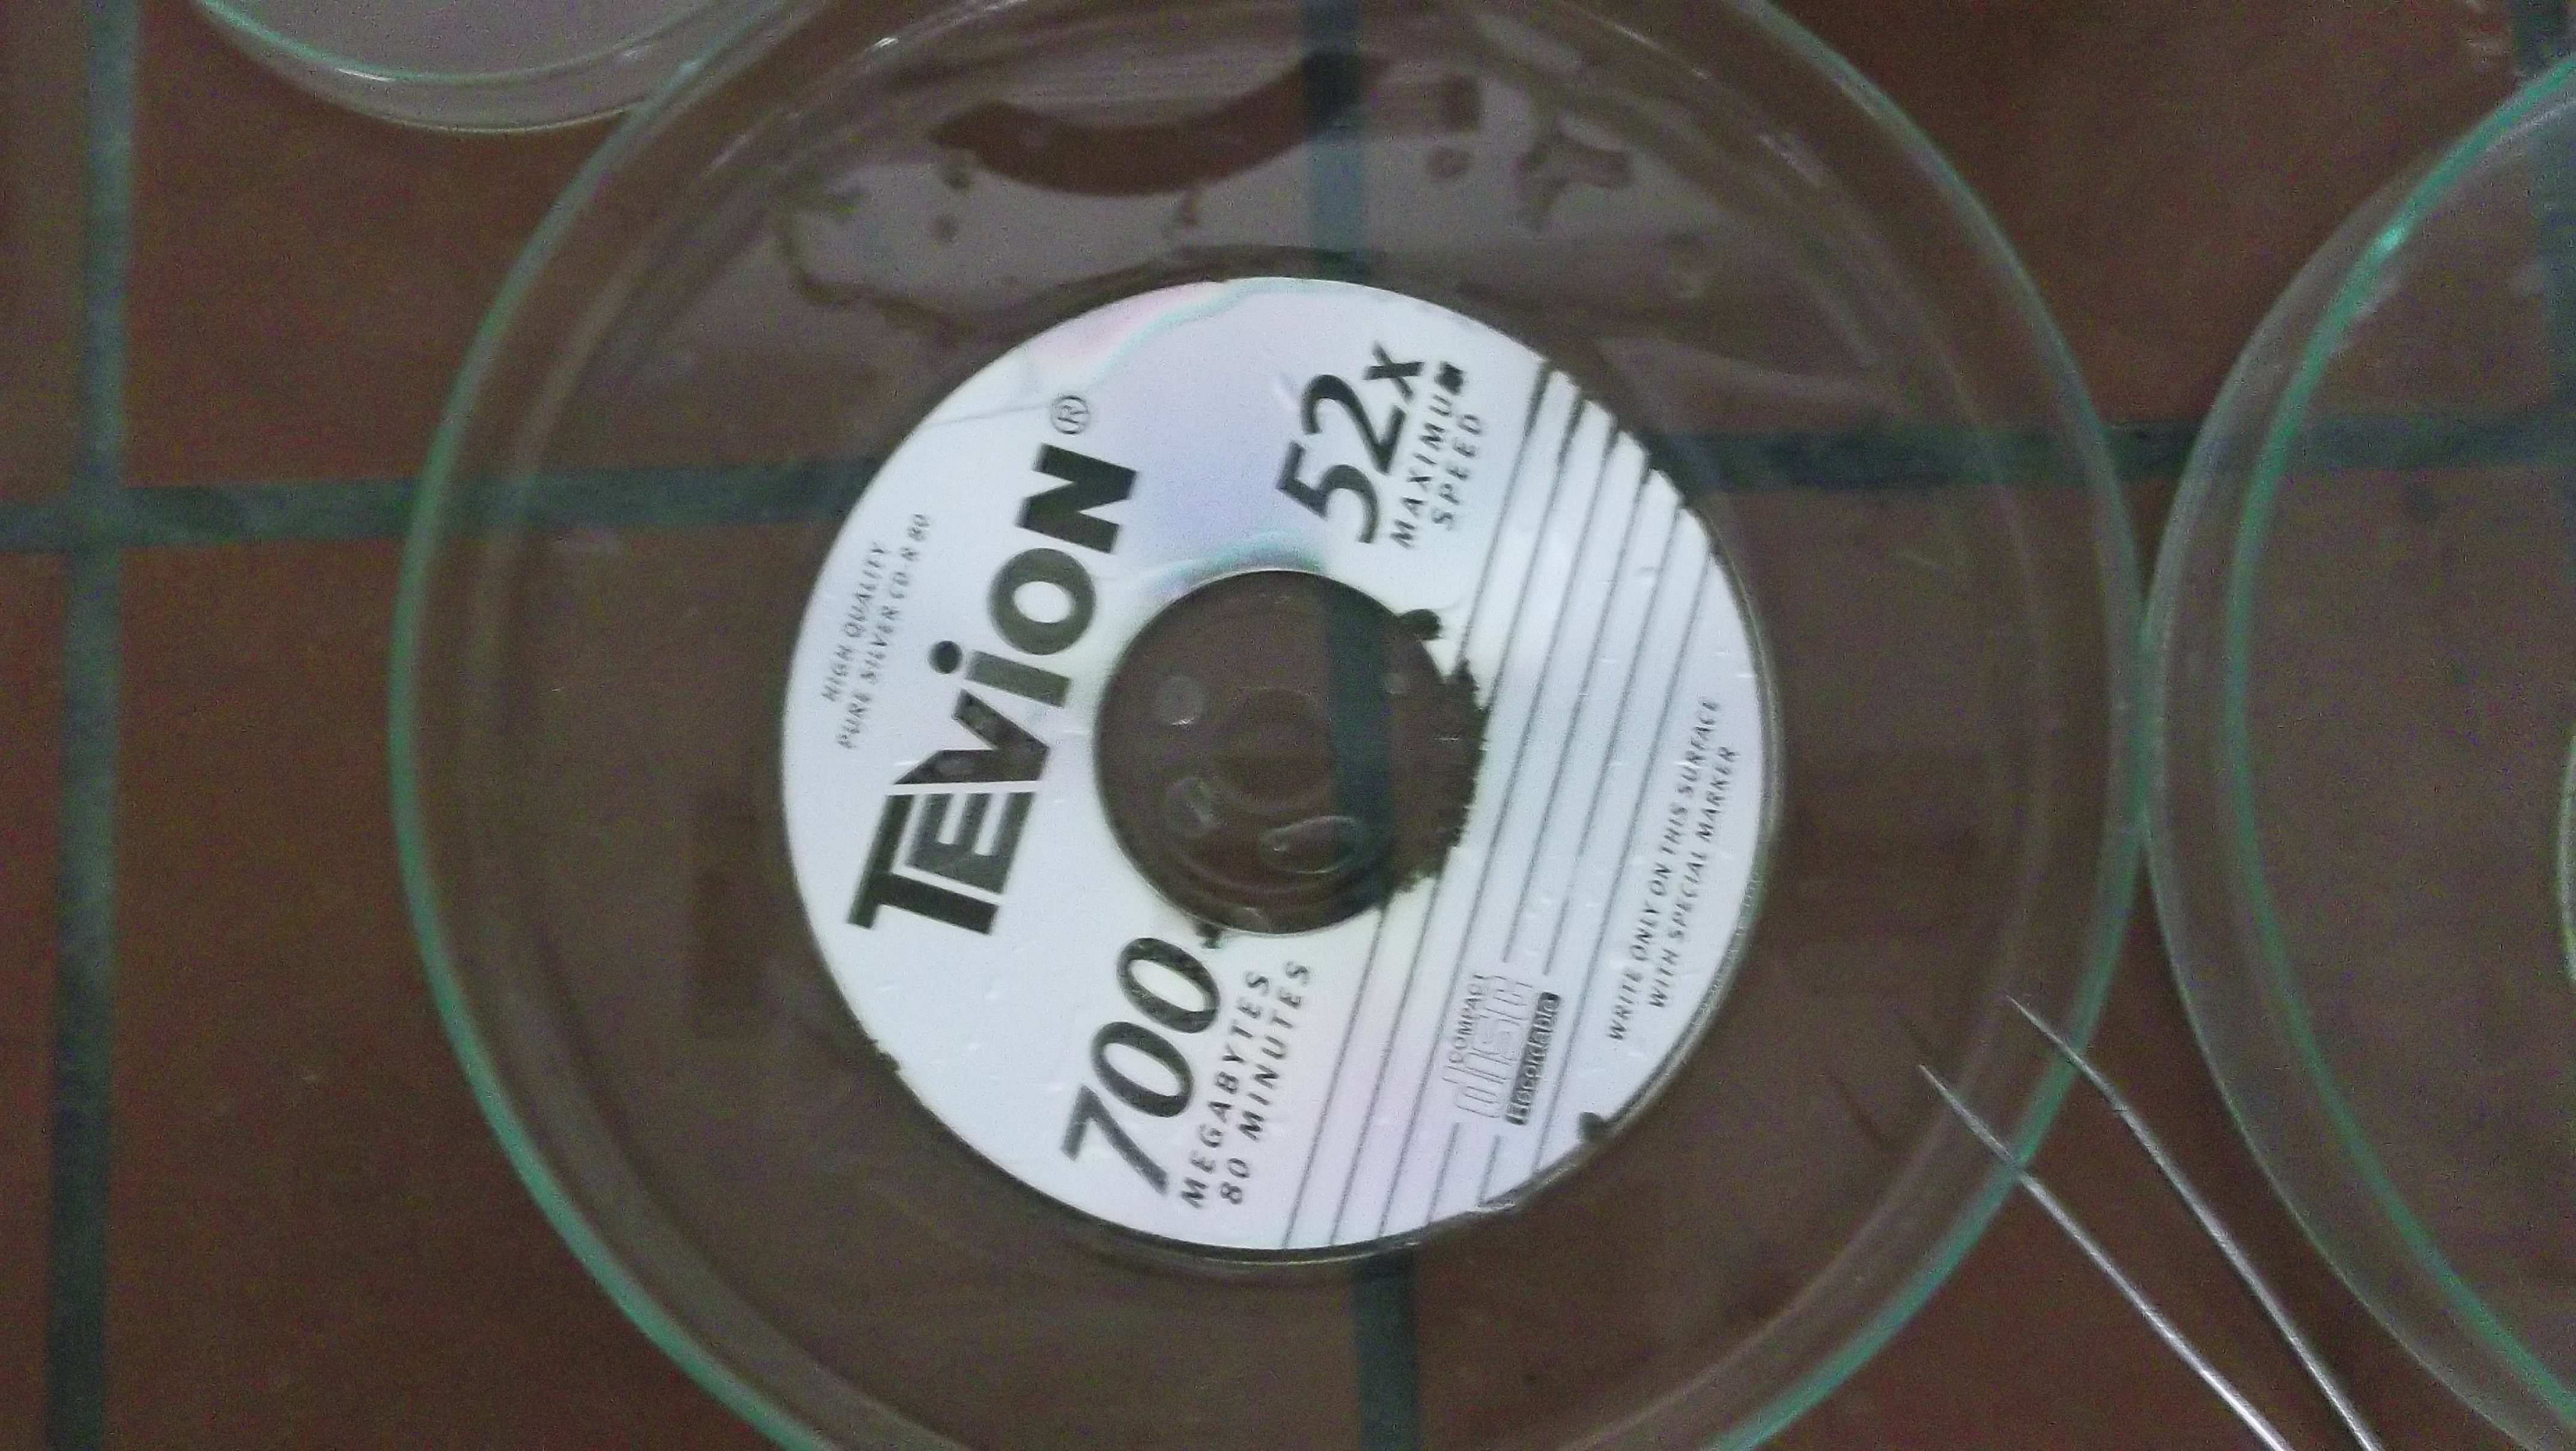
\includegraphics[height=0.1\textheight]{Bilder/Optische_Datentraeger_Die_Compact_Disc/Traegermaterial_Polycarbonat/cdsalpeter.png}
                    \caption[CD in Salpetersäure]{CD in Salpetersäure}
                    \label{fig:cdsalpeter}
                \end{center}
            \end{minipage}
            \hspace{0.025\textwidth}
            \begin{minipage}[t]{0.45\textwidth}
                \begin{center}
                    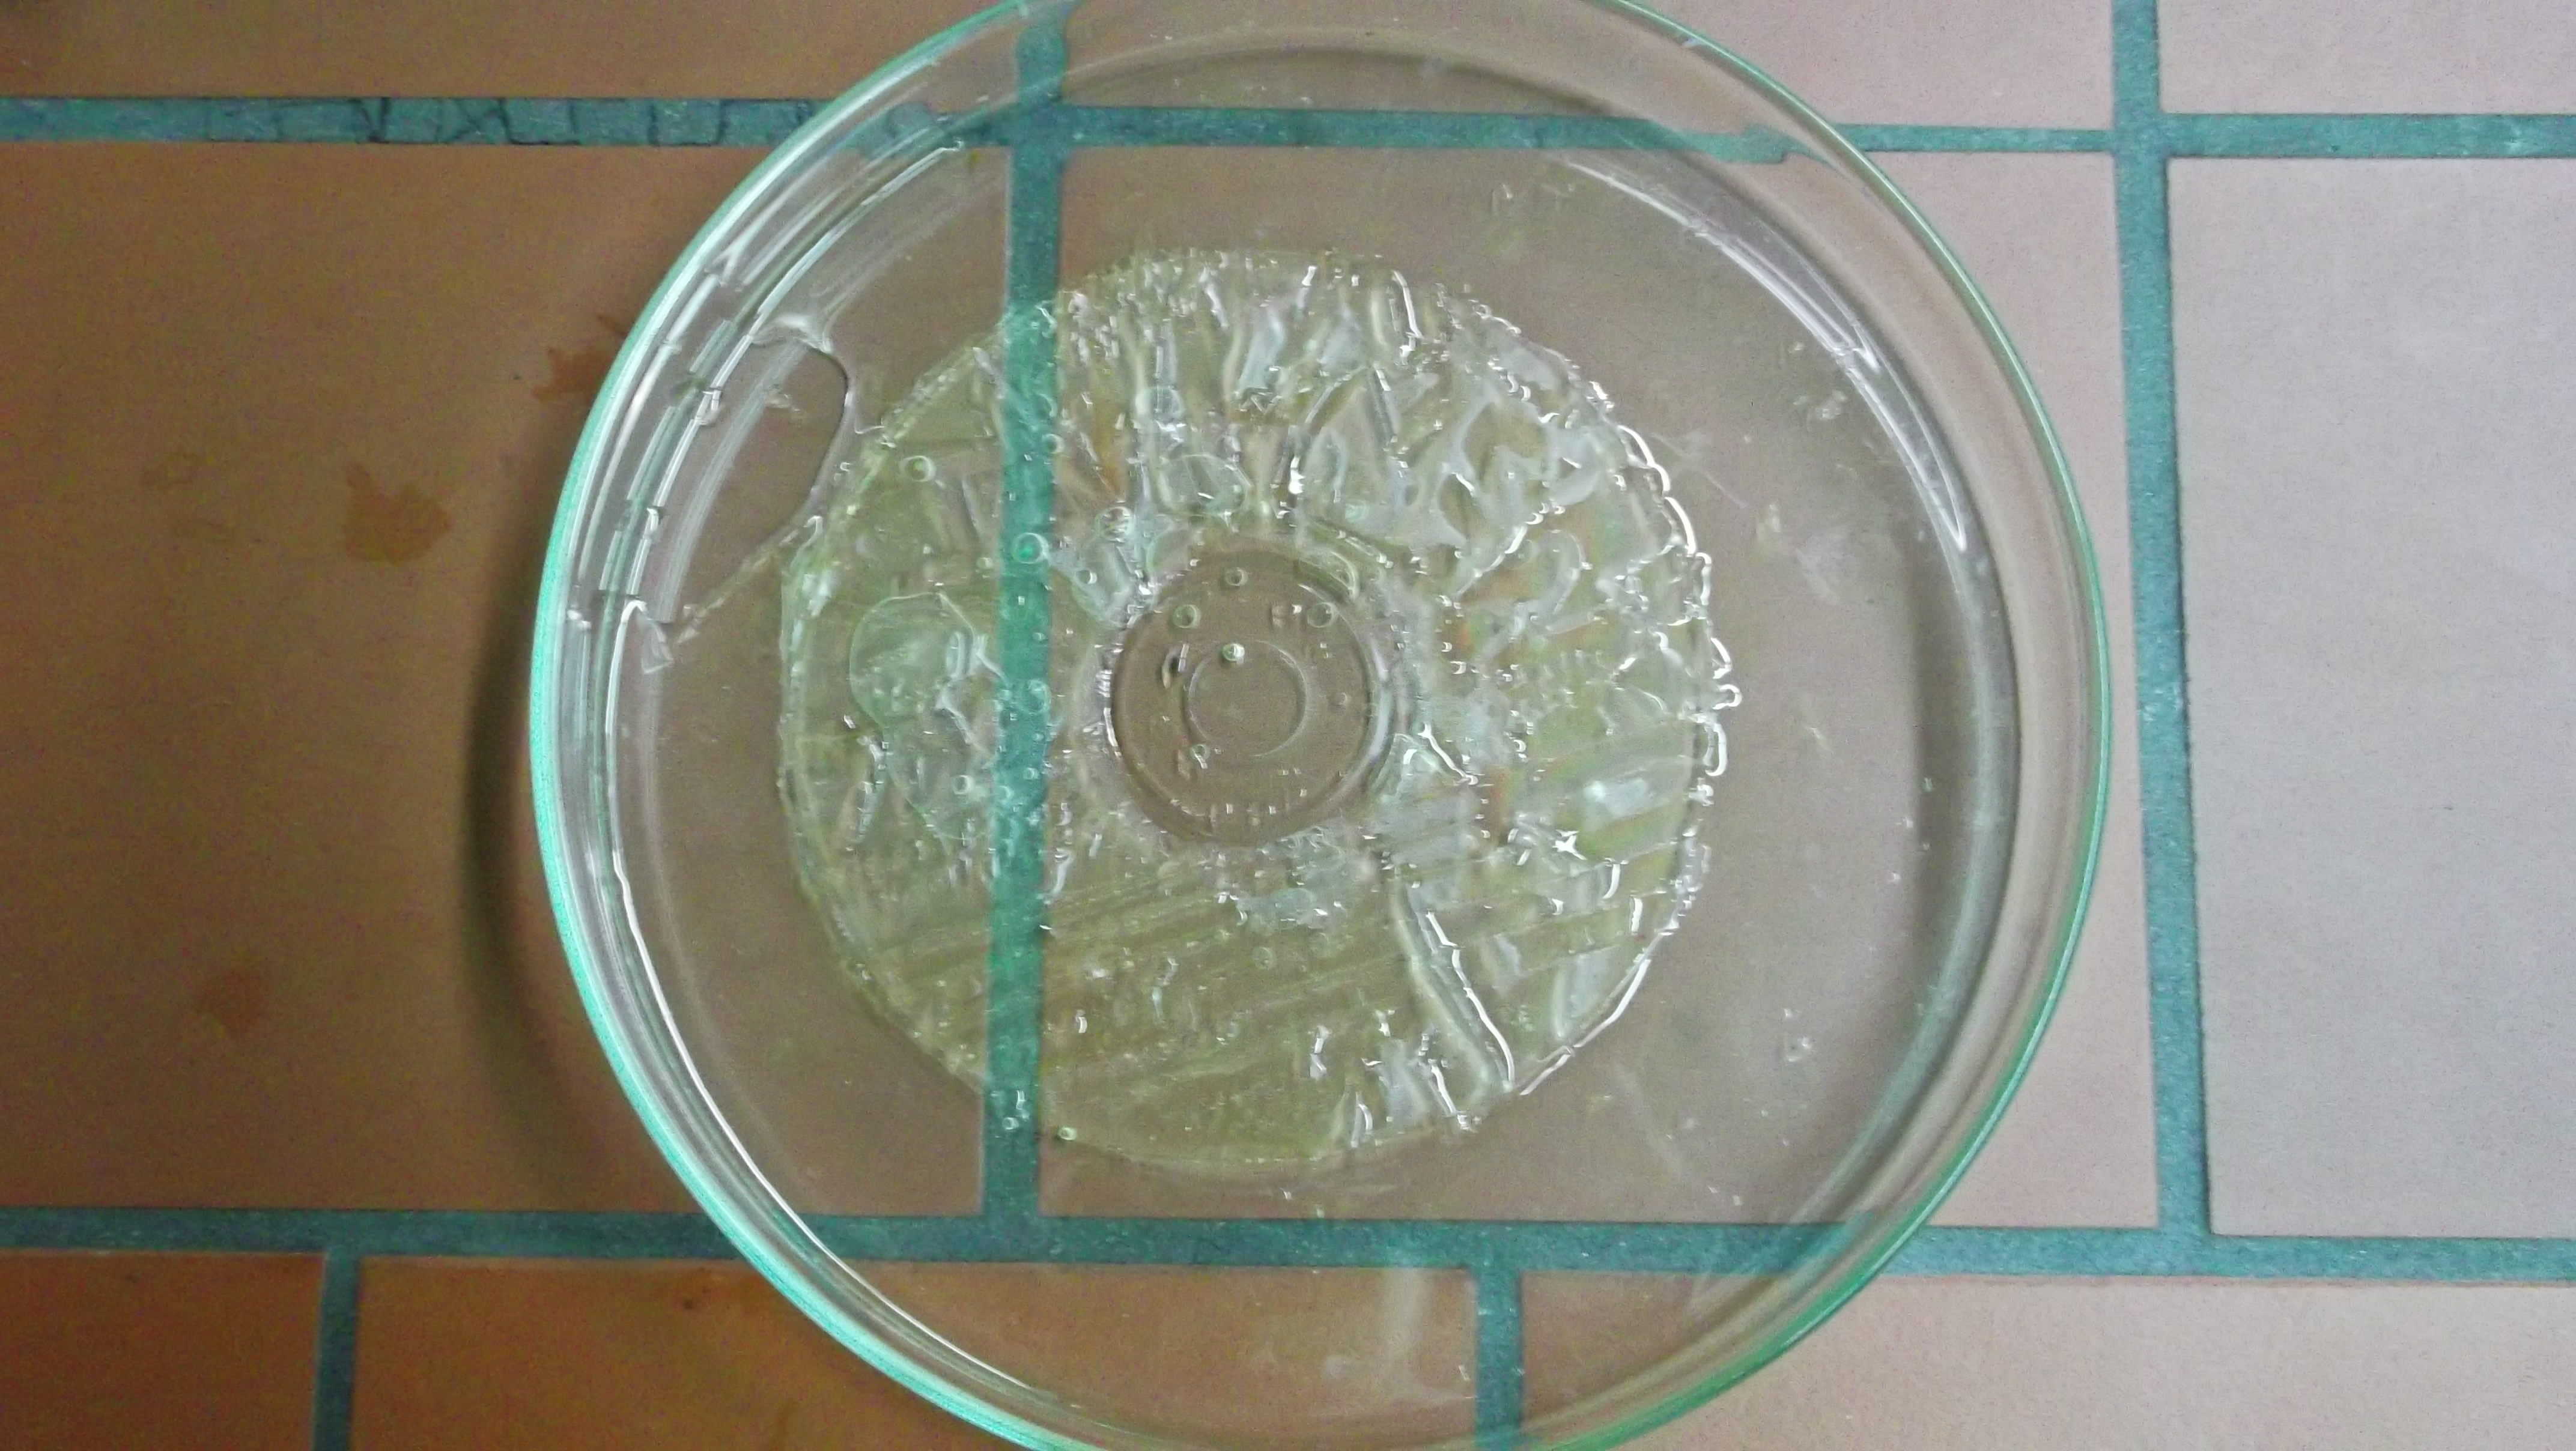
\includegraphics[height=0.1\textheight]{Bilder/Optische_Datentraeger_Die_Compact_Disc/Traegermaterial_Polycarbonat/cdquillt.png}
                    \caption[aufgequollene Lack- und Aluminiumschicht]{\glqq aufgequollene\grqq{} Lack- und Aluminiumschicht}
                    \label{fig:cdquillt}
                \end{center}
            \end{minipage}
        \end{center}
    \end{figure}

    \begin{figure}[H]
        \begin{center}
            \begin{minipage}[t]{0.45\textwidth}
                \begin{center}
                    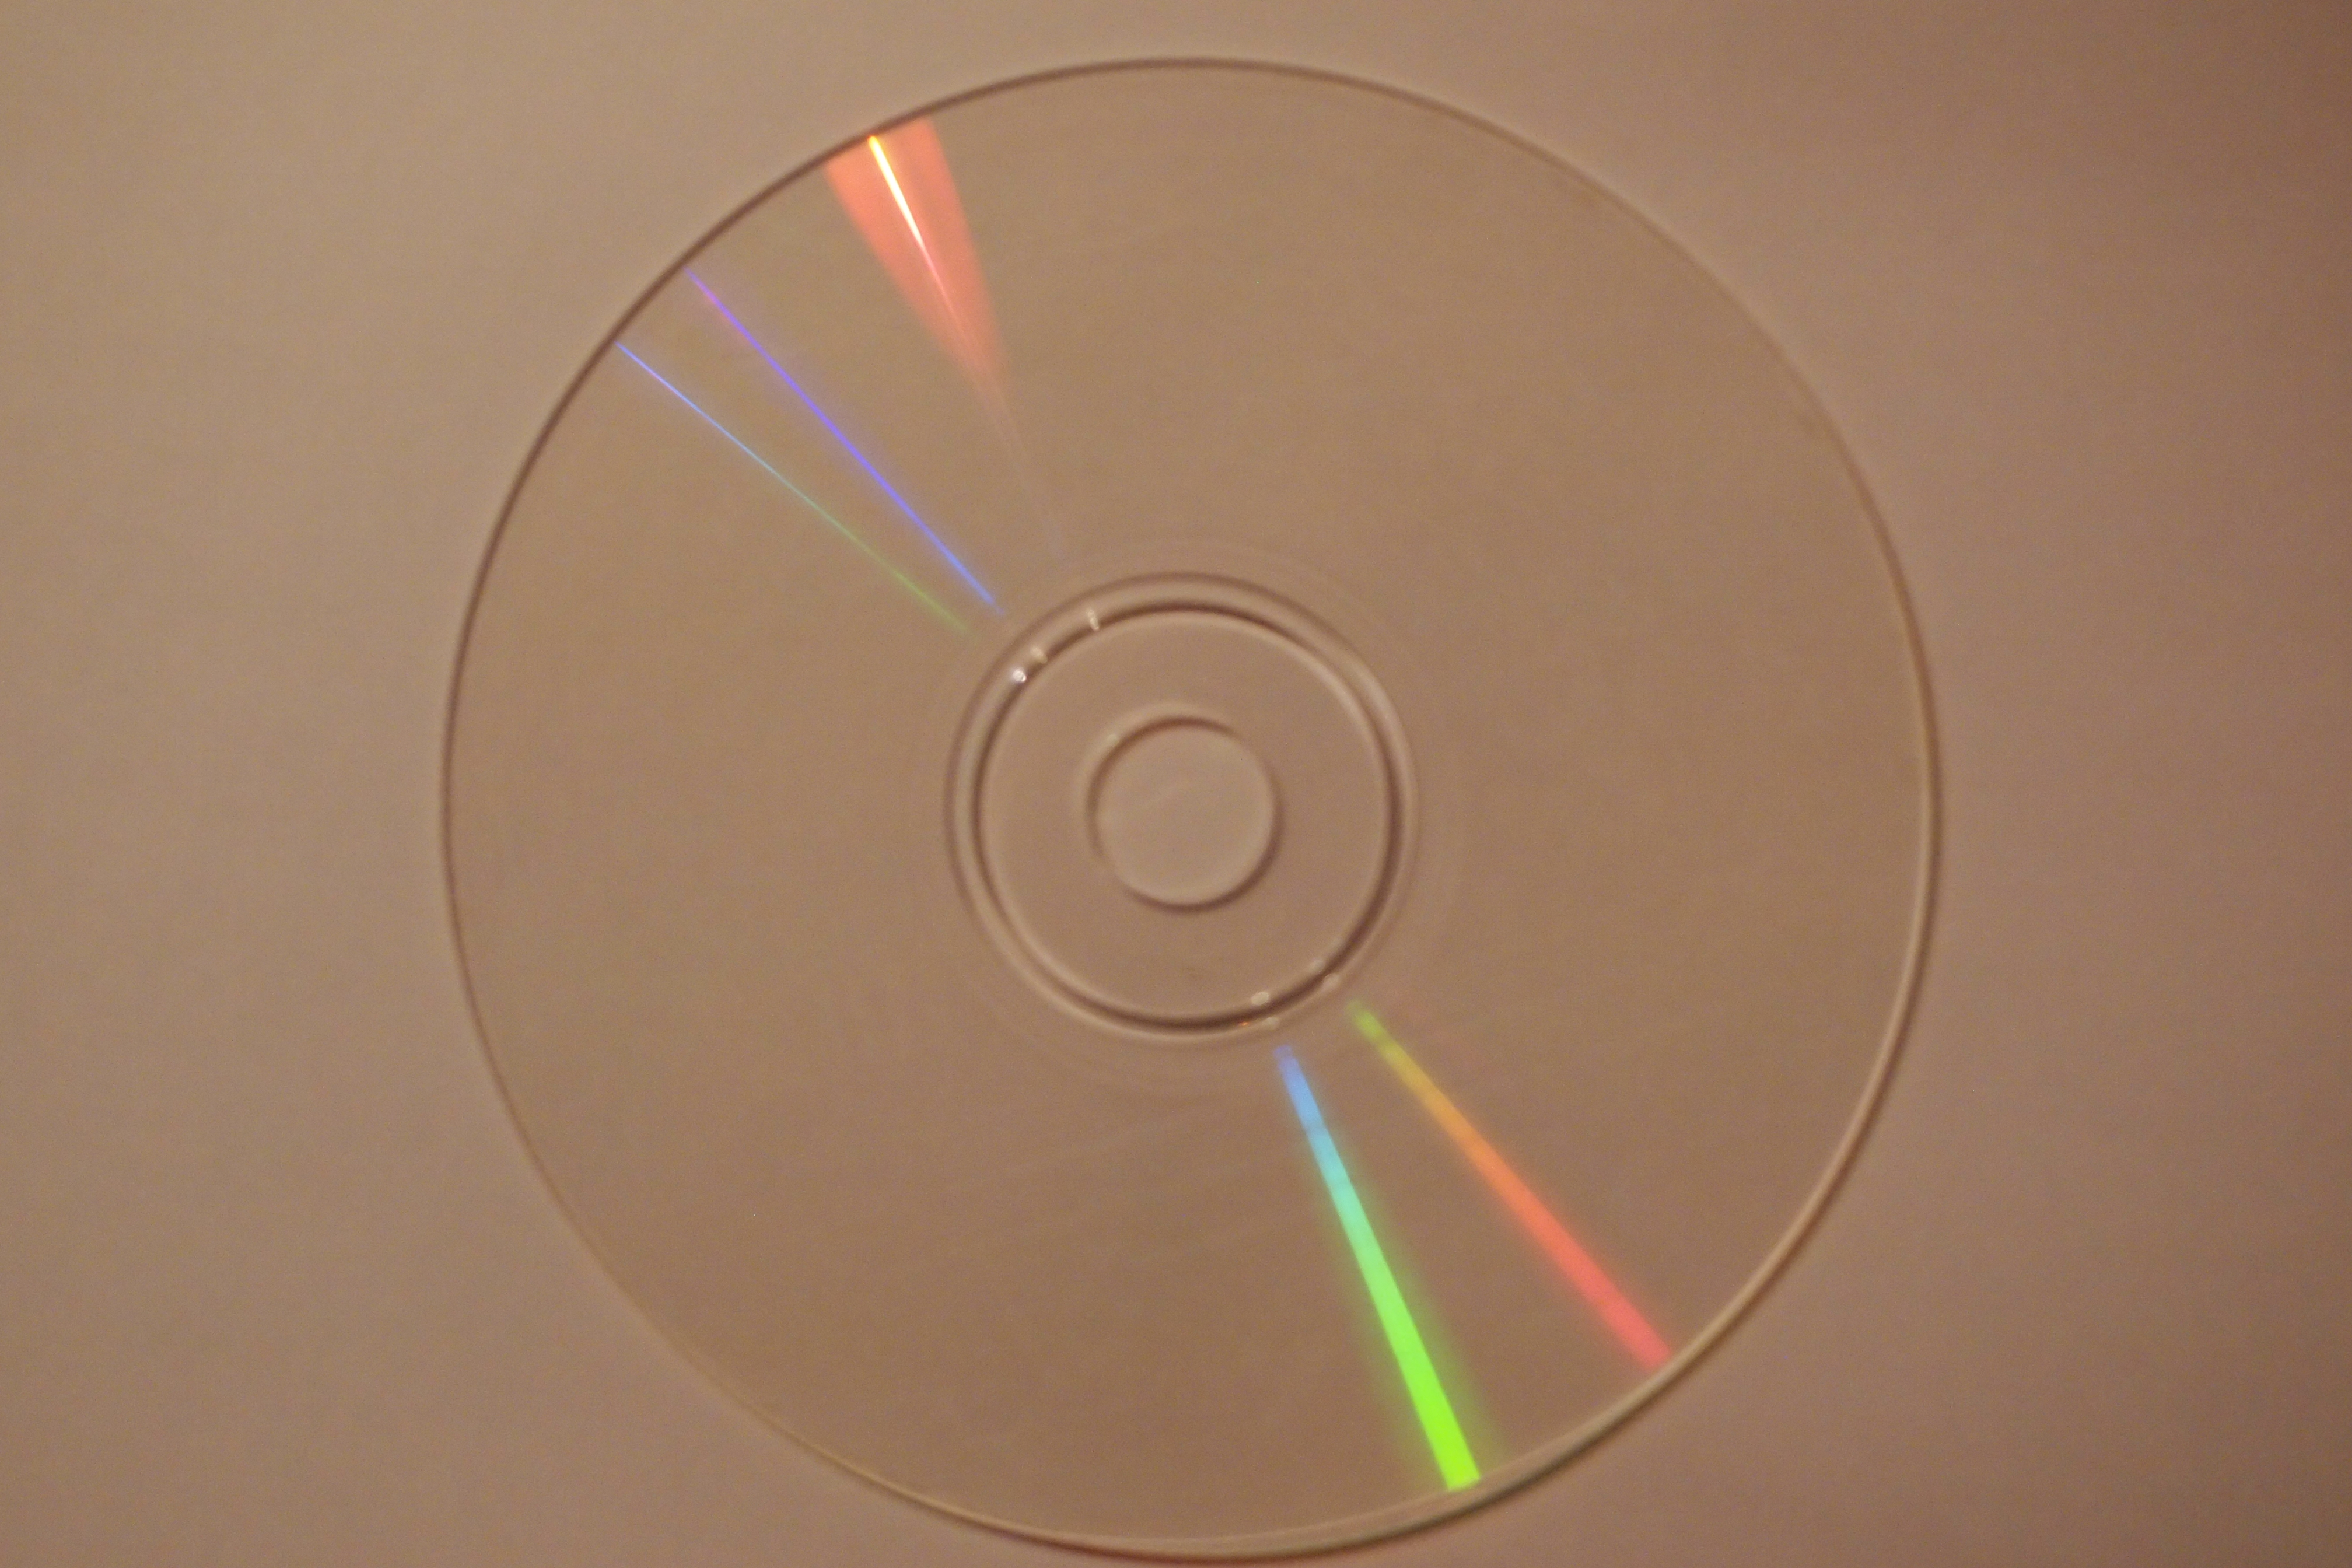
\includegraphics[height=0.1\textheight]{Bilder/Optische_Datentraeger_Die_Compact_Disc/Traegermaterial_Polycarbonat/cdblank.png}
                    \caption[Polycarbonatscheibe]{Polycarbonatscheibe}
                    \label{fig:cdblank}
                \end{center}
            \end{minipage}
            \hspace{0.025\textwidth}
            \begin{minipage}[t]{0.45\textwidth}
                \begin{center}
                    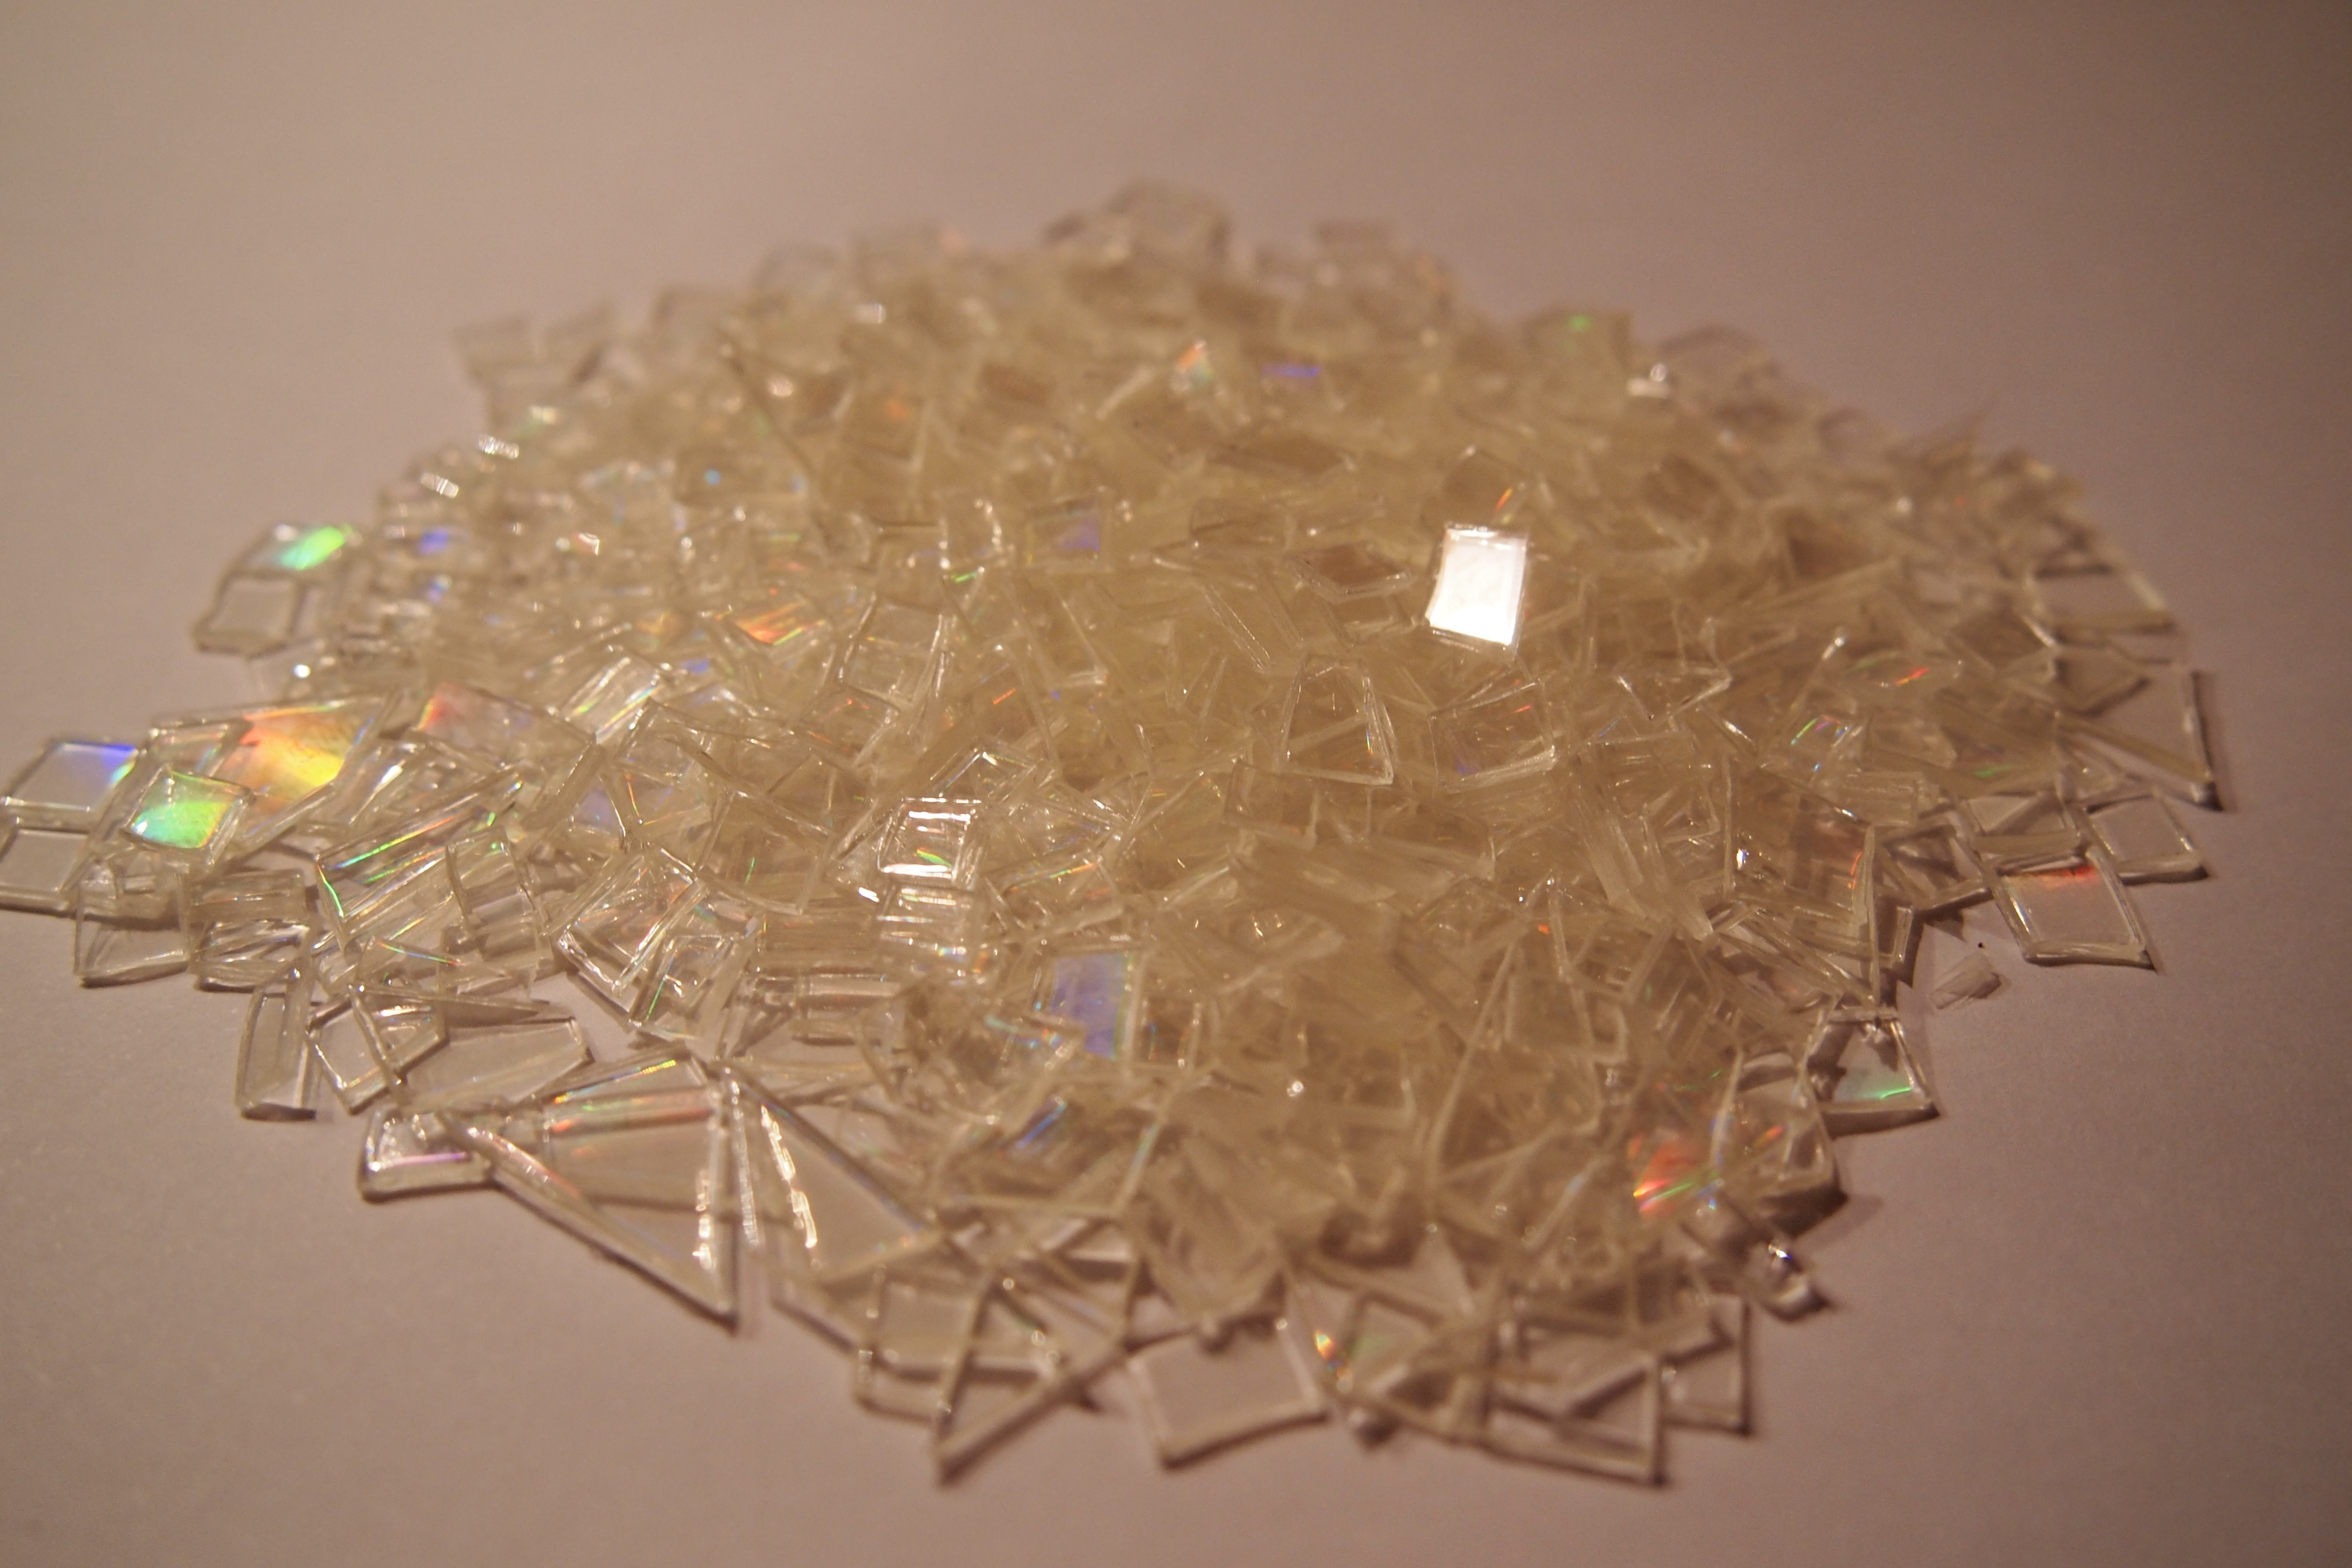
\includegraphics[height=0.1\textheight]{Bilder/Optische_Datentraeger_Die_Compact_Disc/Traegermaterial_Polycarbonat/cdzerschnitten.png}
                    \caption[Polycarbonatstücke]{Polycarbonatstücke}
                    \label{fig:cdzerschnitten}
                \end{center}
            \end{minipage}
        \end{center}
    \end{figure}

    \begin{figure}[H]
        \begin{center}
            \begin{minipage}[t]{0.45\textwidth}
                \begin{center}
                    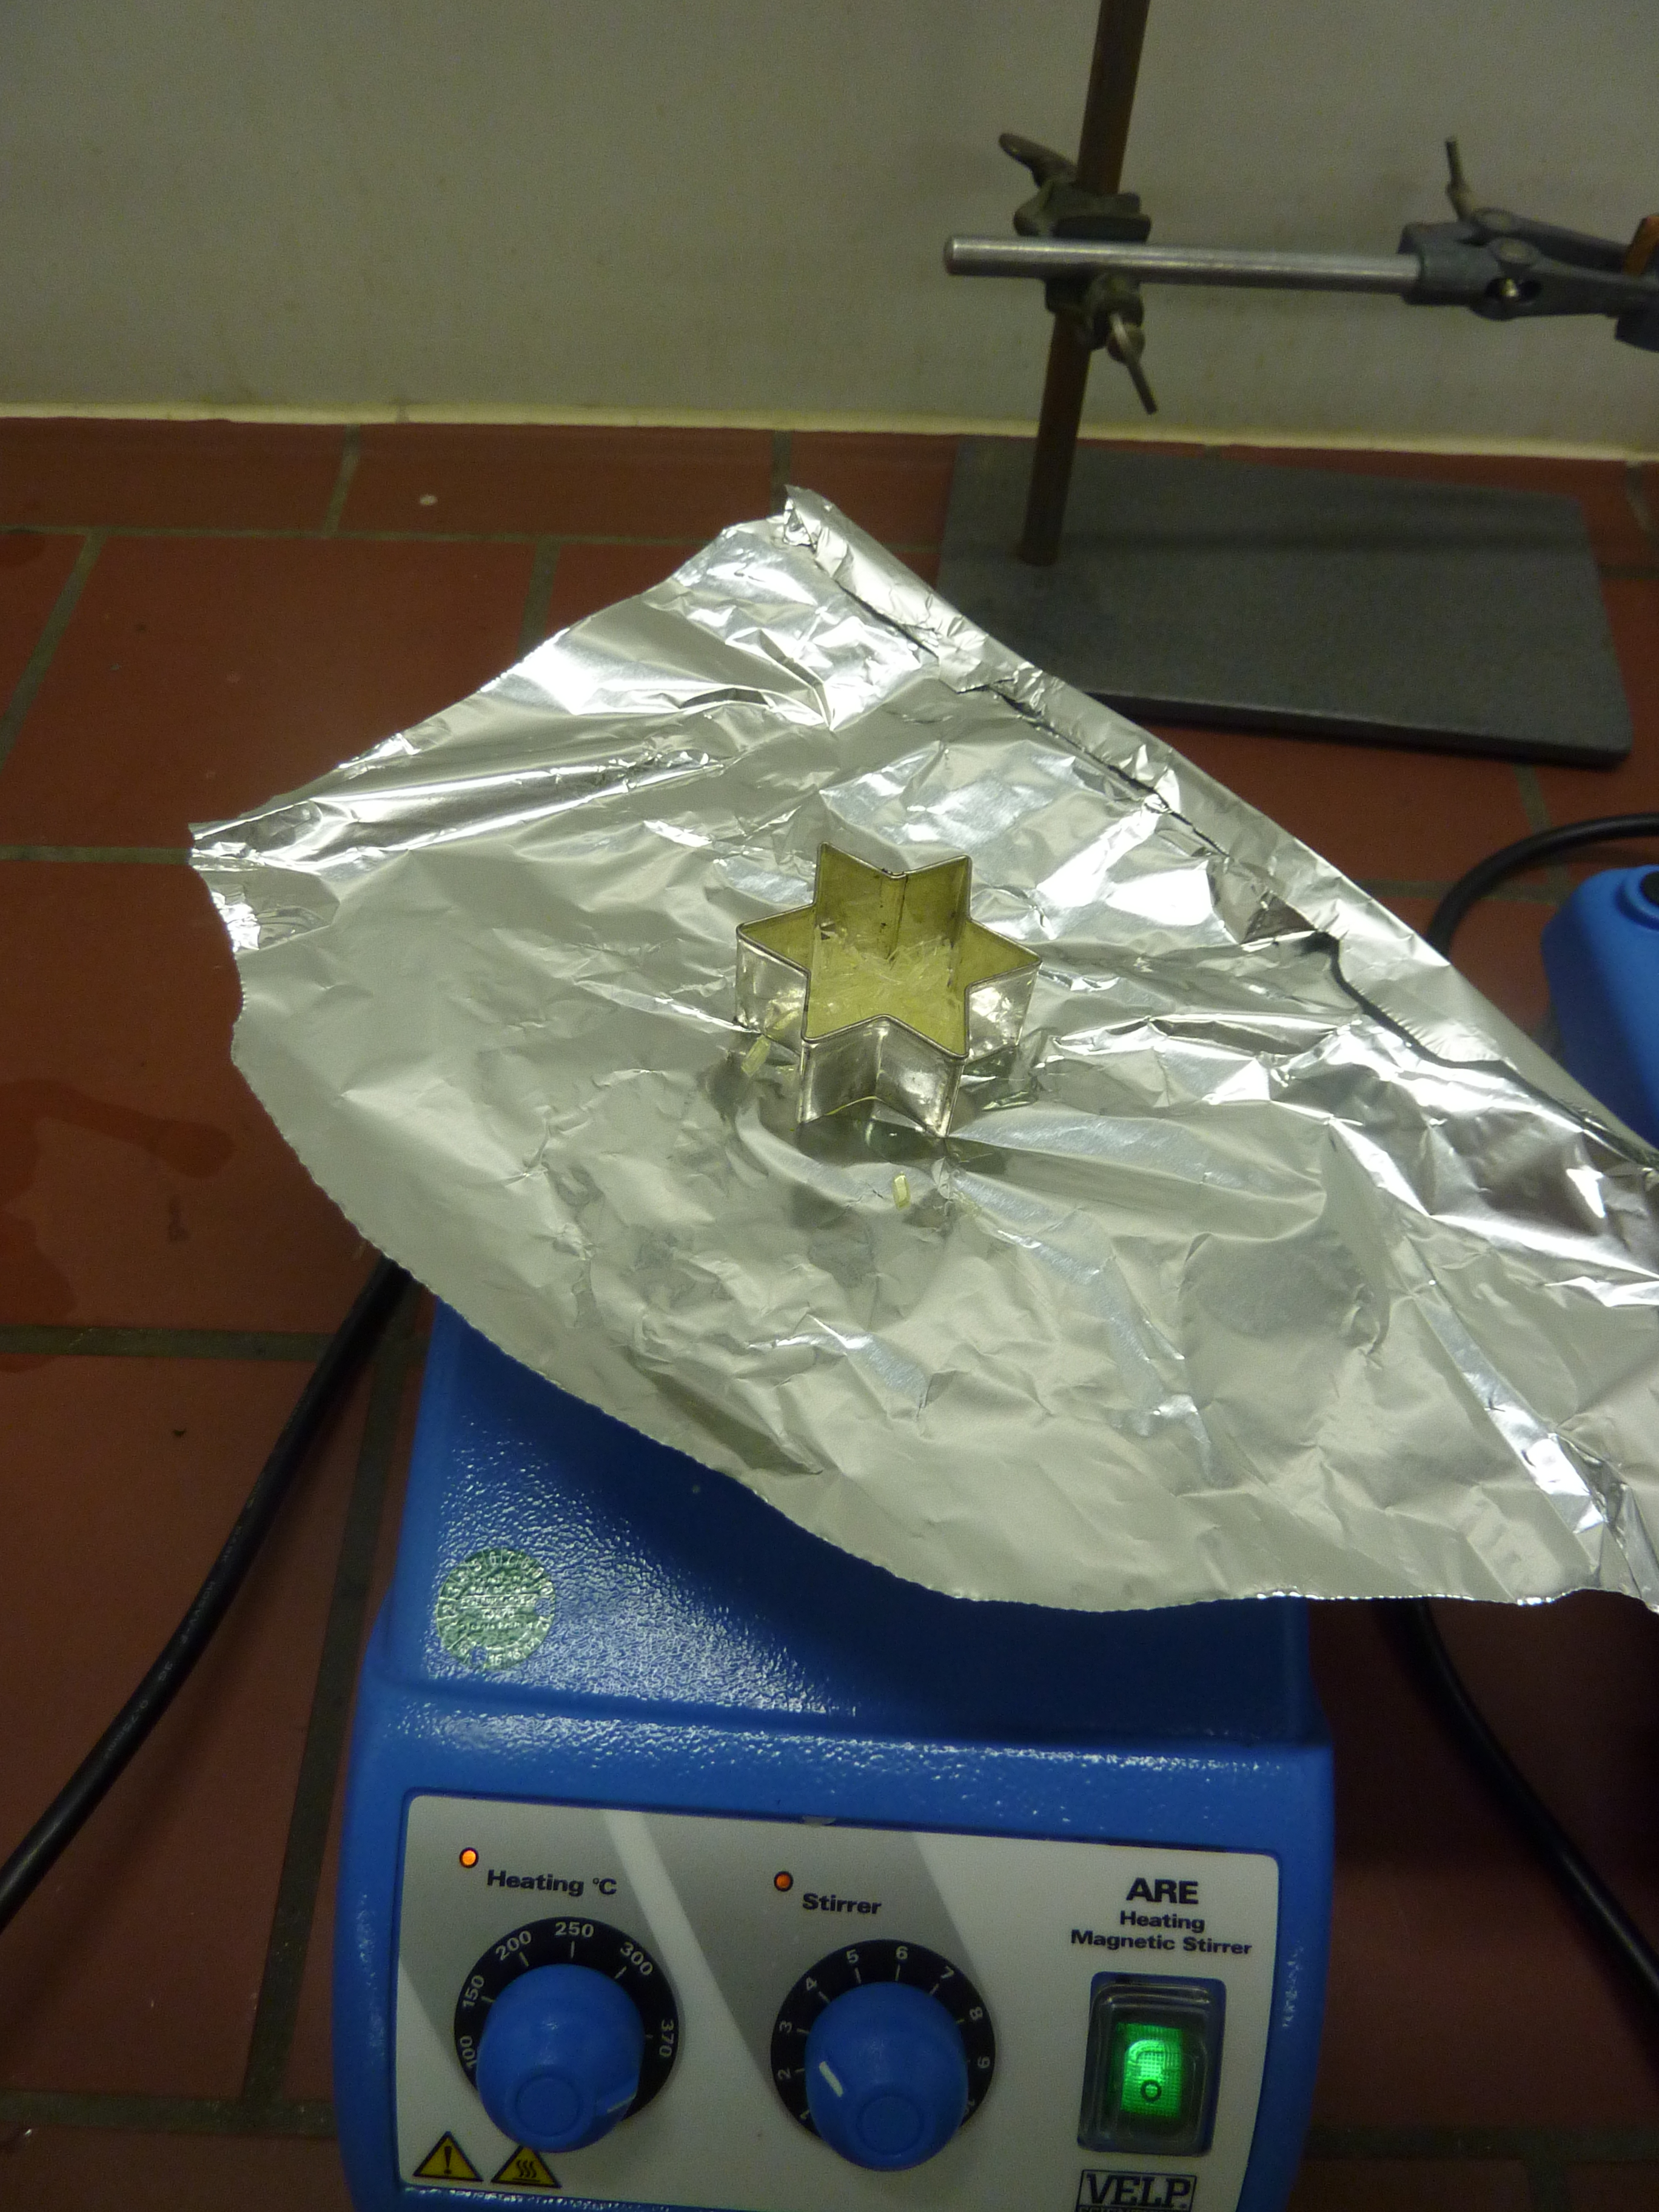
\includegraphics[height=0.1\textheight]{Bilder/Optische_Datentraeger_Die_Compact_Disc/Traegermaterial_Polycarbonat/cdschmelzen.png}
                    \caption[Heizplatte mit Plätzchenform]{Heizplatte mit Plätzchenform}
                    \label{fig:cdschmelzen}
                \end{center}
            \end{minipage}
            \hspace{0.025\textwidth}
            \begin{minipage}[t]{0.45\textwidth}
                \begin{center}
                    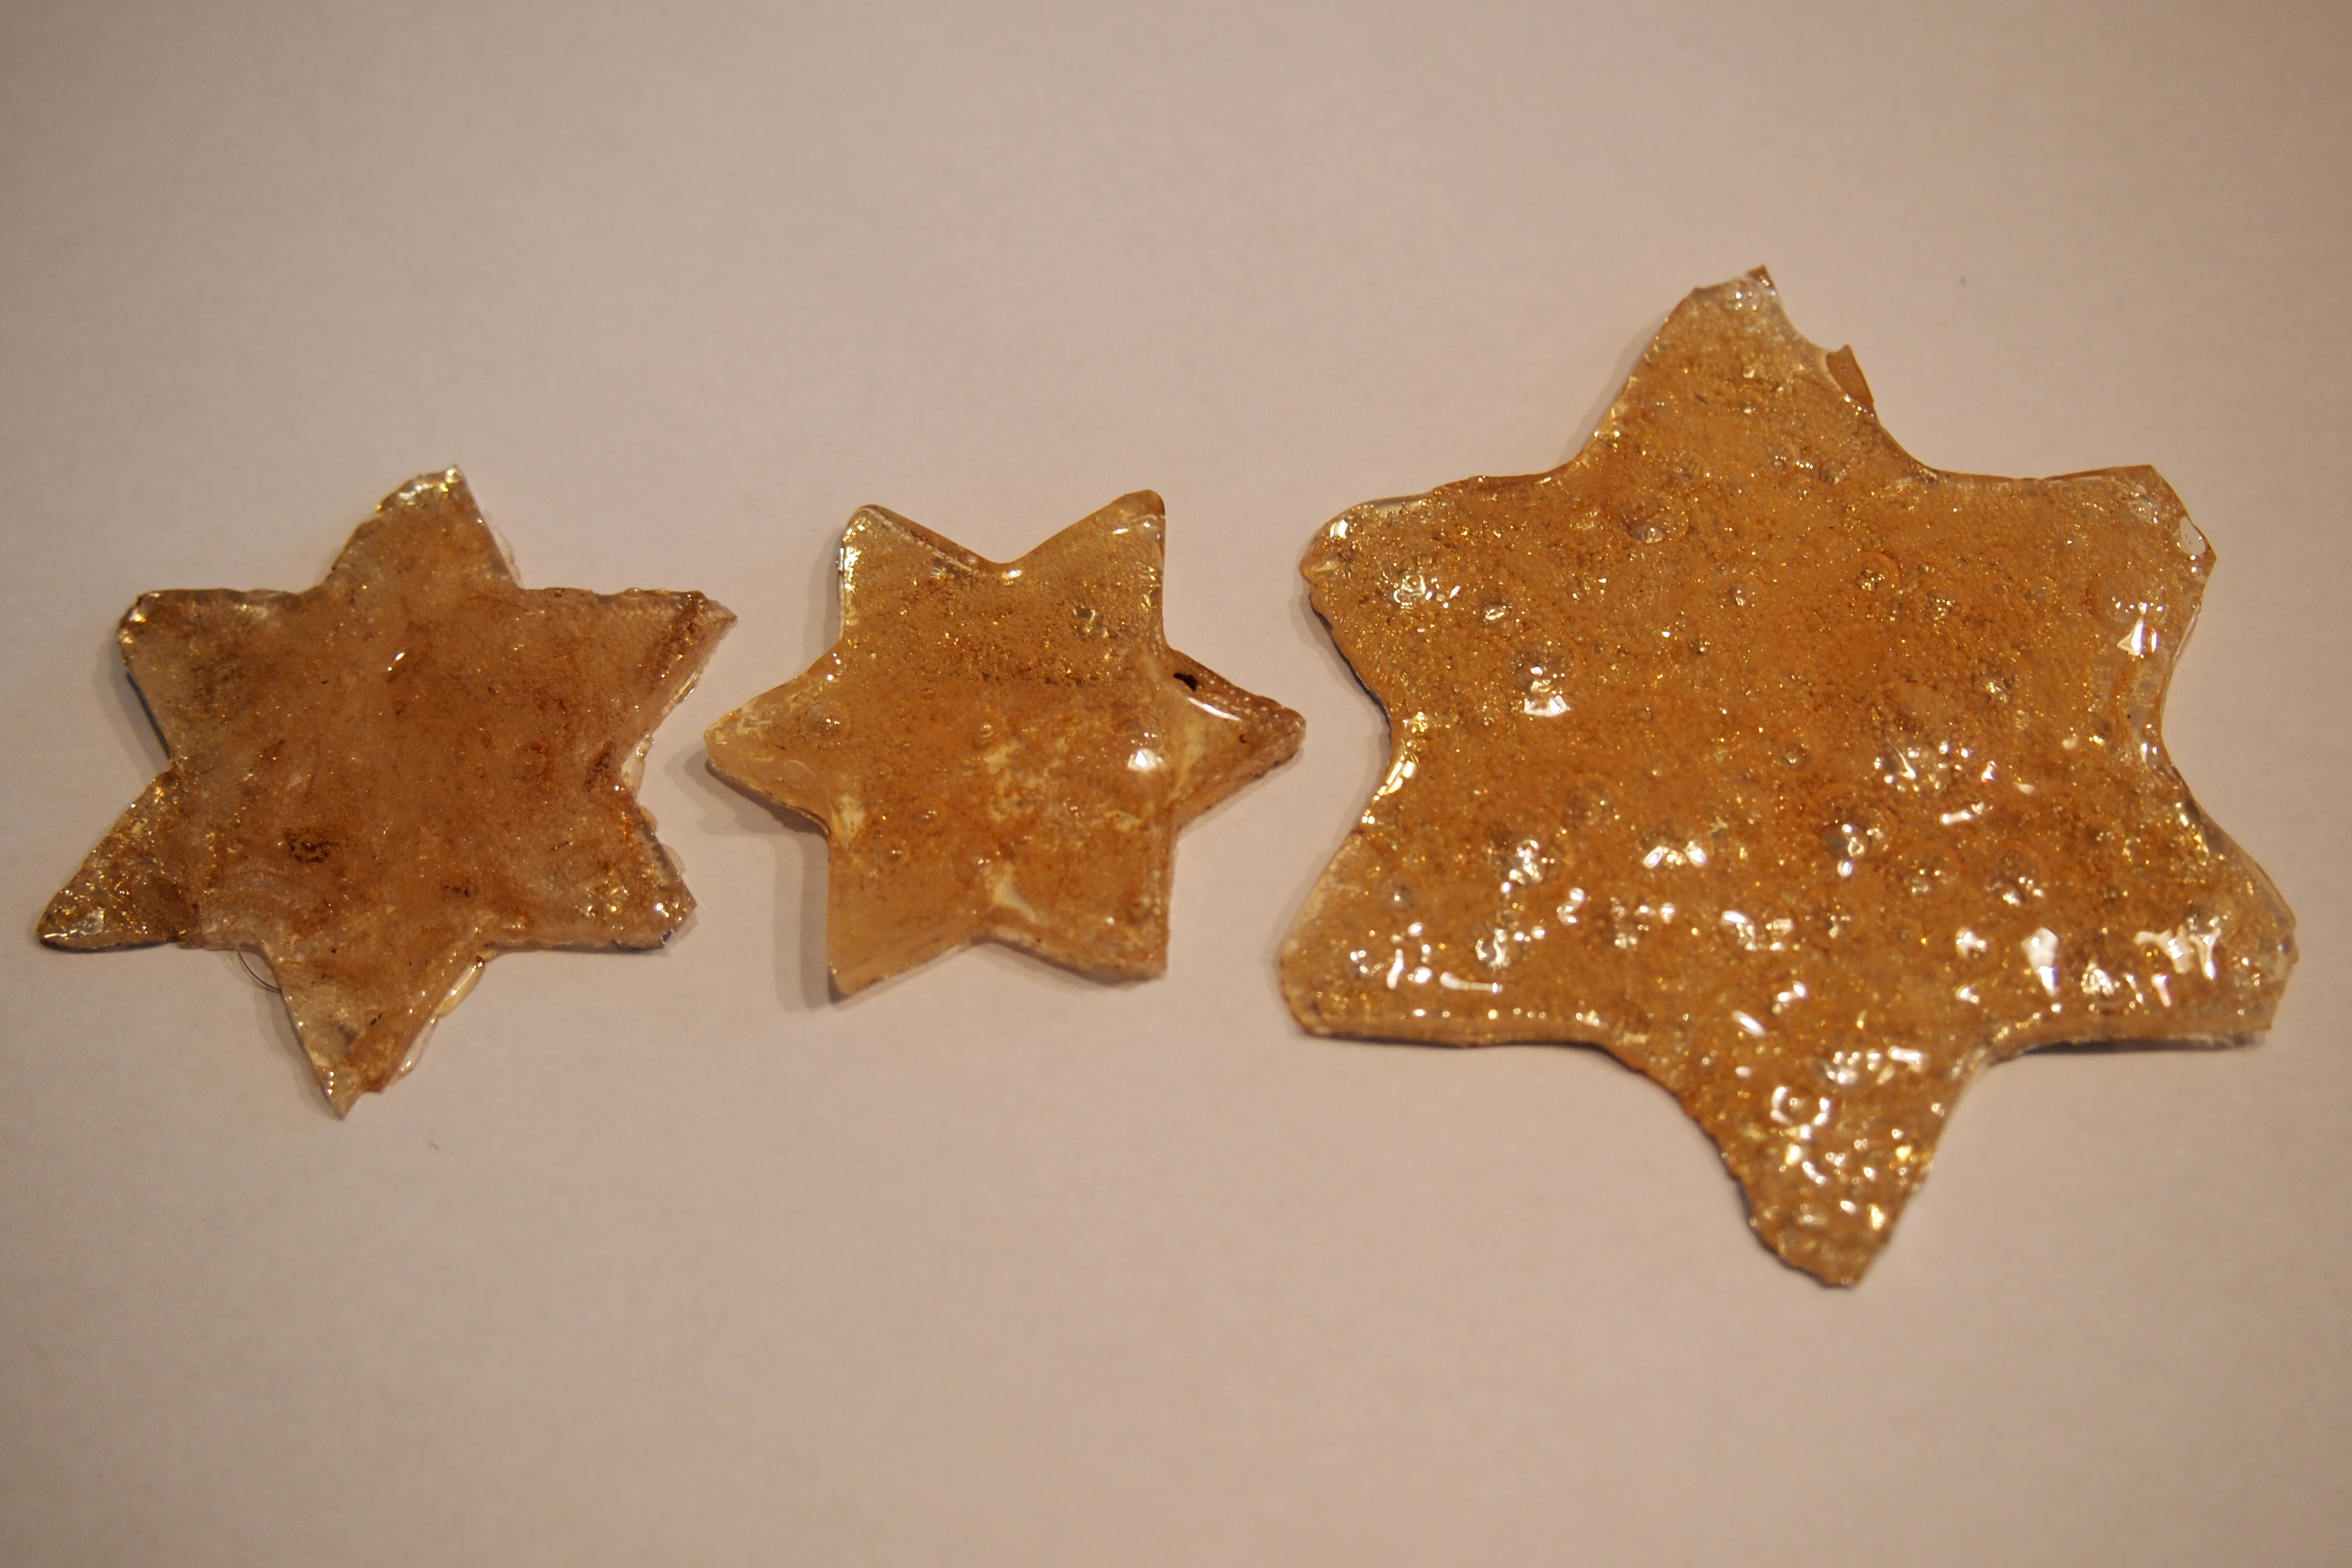
\includegraphics[height=0.1\textheight]{Bilder/Optische_Datentraeger_Die_Compact_Disc/Traegermaterial_Polycarbonat/cdplaetzchen.png}
                    \caption[\glqq Polycarbonatplätzchen\grqq{}]{\glqq Polycarbonatplätzchen\grqq{}}
                    \label{fig:cdplaetzchen}
                \end{center}
            \end{minipage}
        \end{center}
    \end{figure}
}{}

Ergebnisse des Versuchs:
\begin{enumerate*}
    \item Hohe Lichtdurchlässigkeit: Wird die \glqq gehäutete\grqq{} CD in das CD-Laufwerk eines Computers eingelegt, wird diese nicht erkannt, da der Laserstrahl ungehindert durch die Polycarbonatscheibe geht. Dies zeigt, dass die Aluminiumschicht für die Reflexion des Laserstrahls verantwortlich ist.
    \item Einfache Weiterverarbeitung: Die Polycarbonatstücke lassen sich ohne großen Aufwand und innerhalb kurzer Zeit in eine neue Form schmelzen. Die Qualitätsminderung liegt an Verschmutzungen und Lufteinschlüssen, die aufgrund der primitiven Einschmelzmethode unvermeidbar sind.
\end{enumerate*}
